
\section{Neural Networks}
\subsection{Introduction}
\begin{frame}[t]{What is a neural network?}
A neural network is a model that learns how to map fingerprints (in this case, of a molecule) to output quantities (atomization energies, spin-splitting energies).
\visible<2->{\par Nonlinear activation functions make neural networks powerful.}
\visible<3->{\par $\sigma(z)\rightarrow ReLU(z)=$\[ \begin{cases} 
z & z>0 \\
0 & otherwise
\end{cases}
\]}
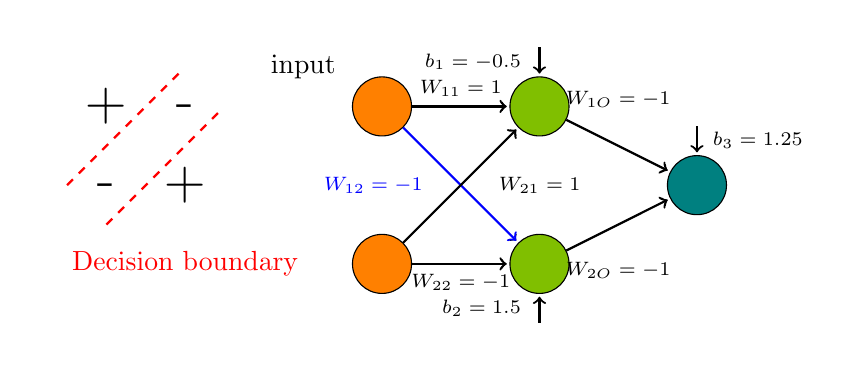
\begin{tikzpicture}[shorten >=1pt,draw=black, x=1cm, y=1 cm,  node distance=0cm]
	\draw[draw=none, use as bounding box](-2,0) rectangle (8,4);
	\clip (-2,-0) rectangle (8,6);
	\def\layersep{2cm}
	
    \tikzstyle{every pin edge}=[<-,shorten <=1pt,thick]
    \tikzstyle{neuron}=[circle,fill=black!25,minimum size=0.75cm ,inner sep=0pt, color=black, draw]
    \tikzstyle{input neuron}=[neuron, fill=green!50!blue!50];
    \tikzstyle{output neuron}=[neuron, fill=green!50!blue];
    \tikzstyle{hidden neuron}=[neuron, fill=green!50!orange];
    \tikzstyle{annot} = [text width=2em, text centered]
    \visible<4->{\node[] (I) at (-1,2) {\huge-};}
    \visible<4->{\node[] (I) at (-1,3) {\huge+};}
    \visible<4->{\node[] (I) at (0,2) {\huge+};}
    \visible<4->{\node[] (I) at (0,3) {\huge-};}
    \visible<5->{\draw[red,thick,dashed] (-1.5,2) -- (0,3.5);}
    \visible<5->{\draw[red,thick,dashed] (-1,1.5) -- (0.5,3);}
    \visible<5->{\node[red] (I) at (0,1) {Decision boundary};}
	\visible<6->{\node[](l) at (1.5, 3.5) {input};}
	\visible<6->{\node[input neuron,fill=orange!100 ] (I-1) at (2.5,1) {$ $};}
	\visible<6->{\node[input neuron,fill=orange!100 ] (I-2) at (2.5,3) {$ $};}
	\visible<6->{\node[hidden neuron,fill=green!50!orange] (H-1) at (4.5,1) {$ $};}
	\visible<6->{\node[hidden neuron,fill=green!50!orange] (H-2) at (4.5,3) {$ $};}
	\visible<6->{\node[output neuron,fill=green!50!blue] (O) at (6.5,2) {$ $};}
	\foreach \dest in {1,2}{     
		\foreach \source in {1,2}{
			\visible<6->{\path[thin,->,black] (I-\source) edge node[font=\scriptsize] {} (H-\dest) ;}}
		}
	\visible<6->{\path[thin,->,black] (H-1) edge node[font=\scriptsize] {} (O);}
	\visible<6->{\path[thin,->,black] (H-2) edge node[font=\scriptsize] {} (O);}
	\visible<7->{\path[thick,->,black, midway, above,black] (I-2) edge node[font=\scriptsize] {$W_{11}=1$} (H-2) ;}
	\visible<7->{\path[thick,->,blue, midway, left,blue] (I-2) edge node[font=\scriptsize, left=10pt] {$W_{12}=-1$} (H-1) ;}
	\visible<7->{\path[thick,->,black, midway, right,black] (I-1) edge node[font=\scriptsize, right=10pt] {$W_{21}=1$} (H-2) ;}
	\visible<7->{\path[thick,->,black, midway, below,black] (I-1) edge node[font=\scriptsize] {$W_{22}=-1$} (H-1) ;}
	\visible<7->{\path[thick,->,black, midway, below,black] (H-1) edge node[font=\scriptsize, below = 10pt] {$W_{2O}=-1$} (O) ;}
	\visible<7->{\path[thick,->,black, midway, below,black] (H-2) edge node[font=\scriptsize, above = 10pt] {$W_{1O}=-1$} (O) ;}
	\visible<7->{\path[thick,->,black, midway, below,black] (4.5,0.25) edge node[font=\scriptsize, left = 3pt] {$b_2=1.5$} (H-1) ;}
	\visible<7->{\path[thick,->,black, midway, below,black] (4.5,3.75) edge node[font=\scriptsize, left = 3pt] {$b_1=-0.5$} (H-2) ;}
	\visible<7->{\path[thick,->,black, midway, below,black] (6.5,2.75) edge node[font=\scriptsize, right = 2pt] {$b_3=1.25$} (O) ;}
\end{tikzpicture}

\end{frame}
\begin{frame}[t]{What do they look like?}
\begin{tikzpicture}[shorten >=1pt,draw=black, x=1cm, y=1 cm,  node distance=0cm]
	\draw[draw=none, use as bounding box](-2,0) rectangle (8,6);
	\clip (-2,-0) rectangle (8,6);
	\def\layersep{2cm}
	
    \tikzstyle{every pin edge}=[<-,shorten <=1pt,thick]
    \tikzstyle{neuron}=[circle,fill=black!25,minimum size=0.5cm ,inner sep=0pt, color=black, draw]
    \tikzstyle{input neuron}=[neuron, fill=green!50!blue!50];
    \tikzstyle{output neuron}=[neuron, fill=green!50!blue];
    \tikzstyle{hidden neuron}=[neuron, fill=green!50!orange];
    \tikzstyle{annot} = [text width=2em, text centered]
	\begin{scope}[x=1cm,y=1cm]
    % Draw the input layer nodes
    \foreach \name / \y in {2,3,4}{
        \only<1>{\node[input neuron,fill=orange!100 ] (I-\name) at (0,\y) {$ $};}}
	 % Draw the hidden layer nodes
	 \only<1>{\foreach \name / \y in {1,2,3,4}{
		 \path[yshift=0.5] node[hidden neuron] (H-\name) at (\layersep,\y+0.5) {\small $ $};
		 \path[yshift=0.5] node[hidden neuron] (H2-\name) at (2*\layersep,\y+0.5) {\small $ $};}}
		%%\path[yshift=0.5] node[hidden neuron] (H3-\name) at (3*\layersep,\y+0.5) {\small $ $};}
%		}
	
	 % Draw the output layer node
	 \only<1>{\node[output neuron,pin={[pin edge={->}]right:\footnotesize Output}] at (2.5*\layersep,3) (O) {$ $};}

	 \foreach \dest in {1,2,3,4}     
		 \foreach \source in {1,2,3,4}
		 {
			 \only<1>{\path[thick,->,gray] (H-\source) edge node[font=\scriptsize] {} (H2-\dest) ;}
		}
 %        \foreach \dest in {2,4,6,8}

	 \end{scope}	             
    \foreach \source in {1,2,3,4}{
           \only<1>{\path[thick,->,gray] (H2-\source) edge node[font=\scriptsize] {} (O) ;}
	}
    \foreach \source in {2,3,4}
		\foreach \dest in {1,2,3,4}  {   
        	\only<1>{\path[thick,->,gray] (I-\source) edge node[font=\scriptsize] {} (H-\dest) ;}
	}

%% call out node 1
\node[circle, black,thick,minimum width = 2.7cm,minimum height = 2.7cm,path picture={\node at (path picture bounding box.center){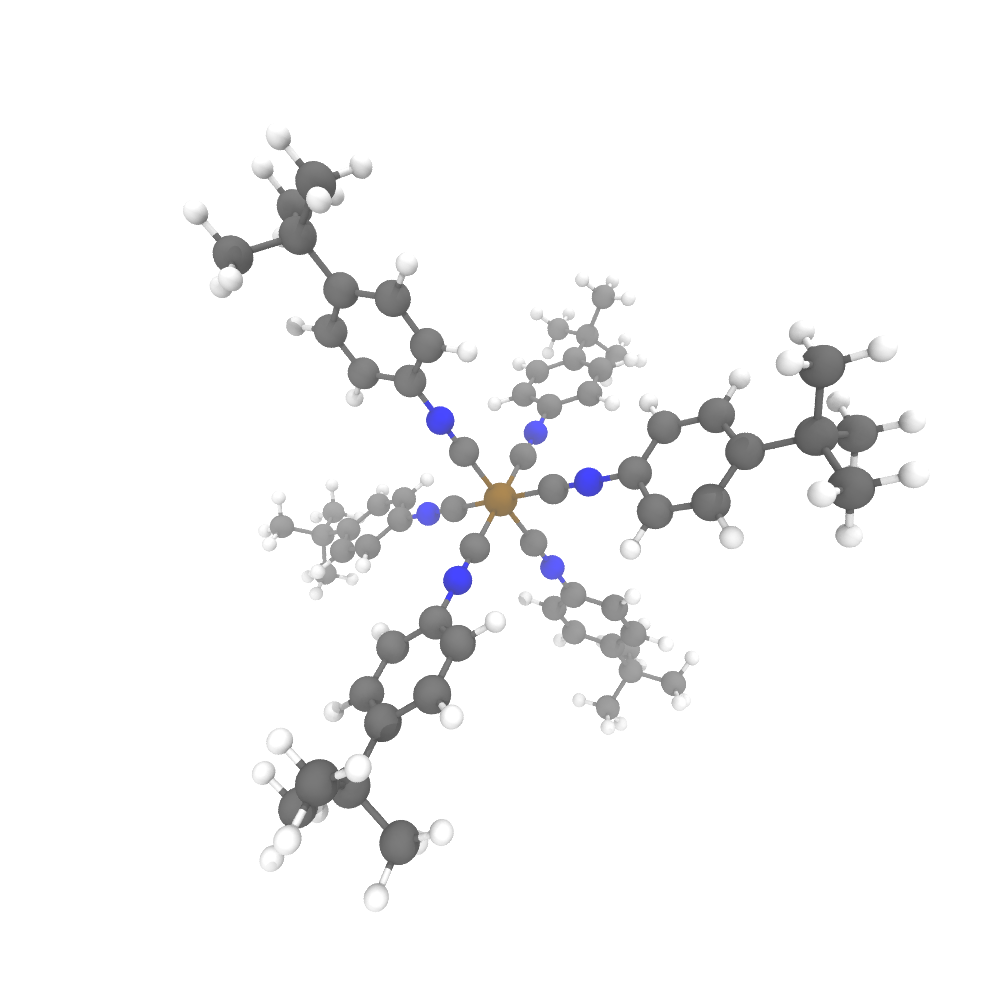
\includegraphics[width=3cm]{representations/images/pisc_trans}}; }] (Xp) at (-1.24,5) {};
\node[] (ll) at (3*\layersep,5) {$\Delta E_{H-L}$};
\node[] (ll) at (2*\layersep,5) {HL2};
\node[] (ll) at (1*\layersep,5) {HL1};

%\only<3->{\node[input neuron,fill=orange!100,opacity=1 ] (I-2) at (0,2) {$ $};}
%\only<4->{\node[hidden neuron,opacity=1 ] (H-2) at (\layersep,2.5) {$ $};}
%\only<5->{\node[hidden neuron,opacity=1 ] (H2-2) at (2*\layersep,2.5) {$ $};}
%\only<6->{\node[hidden neuron,opacity=1 ] (H3-2) at (3*\layersep,2.5) {$ $};}
%\node [circle, fill=red, minimum size = 2cm] (mynode) at (3,3) {};
%\visible<2-3,5->{\node [circle, fill=blue, minimum size = 1cm,opacity=0.5] (mynode) at (3,3) {};}
%\only<2->{\node[circle, fill=green, minimum size = 2cm, below of = mynode] (mynode2) {};}
%\only<2->{\path[draw,very thick,black,->]  (mynode)--(mynode2);}
%    % Annotate the layers
	\node [] (ll) at (-1.25,3) {RAC-155};
\end{tikzpicture}

\end{frame}
\subsection{Mechanics}
\begin{frame}[t]{Backpropagation (chain rule!)}
Back-propagation updates neural network weights $\rightarrow$ example
\visible<2->{\begin{tikzpicture}[shorten >=1pt,draw=black, x=1cm, y=1 cm,  node distance=0cm]
	\draw[draw=gray, use as bounding box](-2,0) rectangle (8,6);
	\clip (-2,-0) rectangle (8,6);
	\def\layersep{2cm}
	\only<7>{\node [] (ll) at (3,5.5) {Loss $\rightarrow L(y)=\sum_{i=1}^{N}((y_i-y_{pred})^2)$ };}
	\only<8->{\node [] (ll) at (3,5.5) {Loss $\rightarrow L(y)=\sum_{i=1}^{N}((y_i-y_{pred})^2)+\lambda(\sum_{l=1}^{L}||W_l||^2)$ };}
	\only<9->{\node [] (ll) at (3,4.5) {We want $\Big(\frac{\partial L}{\partial W_{2,2}}\Big)\rightarrow\sigma_{1,2,3}$ should be differentiable};}
	
    \tikzstyle{every pin edge}=[<-,shorten <=1pt,thick]
    \tikzstyle{neuron}=[circle,fill=black!25,minimum size=0.5cm ,inner sep=0pt, color=black, draw]
    \tikzstyle{input neuron}=[neuron, fill=green!50!blue!50];
    \tikzstyle{output neuron}=[neuron, fill=green!50!blue];
    \tikzstyle{hidden neuron}=[neuron, fill=green!50!orange];
    \tikzstyle{annot} = [text width=2em, text centered]
	\begin{scope}[x=1cm,y=1cm]
    % Draw the input layer nodes
    \foreach \name / \y in {2,3}{
        \visible<1>{\node[input neuron,fill=orange!100 ] (I-\name) at (0,\y) {$ $};}
	\visible<2->{\node[input neuron,fill=orange!100,opacity=0.25 ] (I-\name) at (0,\y) {$ $};}}
	 % Draw the hidden layer nodes
	 \visible<1>{\foreach \name / \y in {1,2,3}{
		 \path[yshift=0.5] node[hidden neuron] (H-\name) at (\layersep,\y+0.5) {\small $ $};
		 \path[yshift=0.5] node[hidden neuron] (H2-\name) at (2*\layersep,\y+0.5) {\small $ $};}}
		%%\path[yshift=0.5] node[hidden neuron] (H3-\name) at (3*\layersep,\y+0.5) {\small $ $};}
%		}
		
	  \visible<2->{\foreach \name / \y in {1,2,3}{
		 \path[yshift=0.5] node[hidden neuron, opacity = 0.25] (H-\name) at (\layersep,\y+0.5) {\small $ $};
		 \path[yshift=0.5] node[hidden neuron, opacity = 0.25] (H2-\name) at (2*\layersep,\y+0.5) {\small $ $};}}
	 % Draw the output layer node
	 \visible<1>{\node[output neuron,pin={[pin edge={->}]right:\footnotesize Output}] at (2.5*\layersep,2.5) (O) {$ $};}
	\visible<2->{\node[output neuron, opacity=0.25,pin={[pin edge={->}]right:\footnotesize Output}] at (2.5*\layersep,2.5) (O) {$ $};}

	 \foreach \dest in {1,2,3}     
		 \foreach \source in {1,2,3}
		 {
			 \visible<1>{\path[thick,->,gray] (H-\source) edge node[font=\scriptsize] {} (H2-\dest) ;}\
			\visible<2->{\path[thin,->,gray] (H-\source) edge node[font=\scriptsize] {} (H2-\dest) ;}
%			 \path[thick,->,gray] (H2-\source) edge node[font=\scriptsize] {} (H3-\dest) ;
		}
 %        \foreach \dest in {2,4,6,8}

	 \end{scope}	             
    \foreach \source in {1,2,3}{
           \visible<1>{\path[thick,->,gray] (H2-\source) edge node[font=\scriptsize] {} (O) ;}
	\visible<2->{\path[thin,->,gray] (H2-\source) edge node[font=\scriptsize] {} (O) ;}}
    \foreach \source in {2,3}
		\foreach \dest in {1,2,3}  {   
        	\visible<1>{\path[thick,->,gray] (I-\source) edge node[font=\scriptsize] {} (H-\dest) ;}
	\visible<2->{\path[thin,->,gray] (I-\source) edge node[font=\scriptsize] {} (H-\dest) ;}}

%% call out node 1
%\node[circle, black,thick,minimum width = 2.7cm,minimum height = 2.7cm,path picture={\node at (path picture bounding box.center){\includegraphics[width=3cm]{representations/images/pisc_trans}}; }] (Xp) at (-1.24,5) {};
%\node[] (ll) at (3*\layersep,5) {$\Delta E_{H-L}$};

\visible<3->{\node[input neuron,fill=orange!100,opacity=1 ] (I-2) at (0,2) {x};}
\visible<3->{\node [] (ll) at (0,0.5) {Input};}
\visible<4->{\path[thick,->,gray] (I-2) edge node[font=\scriptsize] {} (H-1) ;}
\visible<4->{\node[hidden neuron,opacity=1 ] (H-1) at (\layersep,1.5) {$\sigma_{1}$};}
\visible<4->{\node [] (ll) at (\layersep,0.5) {HL1};}
\visible<5->{\path[thick,->,gray] (H-1) edge node[font=\scriptsize] {} (H2-2) ;}
\visible<5->{\node[hidden neuron,opacity=1 ] (H2-2) at (2*\layersep,2.5) {$\sigma_{2}$};}
\visible<5->{\node [] (ll) at (2*\layersep,0.5) {HL2};}
\visible<5->{\path[thick,->,gray] (H2-2) edge node[font=\scriptsize] {} (O) ;}
\visible<6->{\node[output neuron,opacity=1] (O) at (2.5*\layersep,2.5) {$\sigma_3$};}
\visible<6->{\node [] (ll) at (2.5*\layersep,0.5) {OL};}
%\node [circle, fill=red, minimum size = 2cm] (mynode) at (3,3) {};
%\visible<2-3,5->{\node [circle, fill=blue, minimum size = 1cm,opacity=0.5] (mynode) at (3,3) {};}
%\only<2->{\node[circle, fill=green, minimum size = 2cm, below of = mynode] (mynode2) {};}
%\only<2->{\path[draw,very thick,black,->]  (mynode)--(mynode2);}
%    % Annotate the layers
	\node [] (ll) at (-1.25,2.5) {RAC-155};
\end{tikzpicture}}

\end{frame}
\begin{frame}[t]{SGD and training process}
\visible<1->{Backpropagation is normally used to find the gradients. Since all of the gradients are made easy to find with backpropagation, they can be updated with gradient descent:}
\visible<2->{$$W = W-\eta *\Big(\frac{\partial Loss}{\partial W}\Big)$$}
\visible<3->{In gradient descent, loss term calculated from training data $\rightarrow$ if you train for the same number of epochs (number of rounds your NN sees the training data), you will get the same result. \textbf{Gets stuck in local minima!}}
\visible<4->{$$GD\rightarrow\Big(\frac{\partial Loss}{\partial W}\Big)\rightarrow all\:training\:data$$}
\visible<5->{$$SGD\rightarrow\Big(\frac{\partial Loss}{\partial W}\Big)\rightarrow one/few\:examples\rightarrow MUCH\:noisier!\rightarrow less\:stuck$$}
\end{frame}
\begin{frame}[t]{Other types of layers}
\visible<1->{\textbf{Input}$\rightarrow$ layers on the NN where inputs are fed}\\
\visible<2->{\textbf{Hidden}$\rightarrow$ layers between the input and output nodes, helps to create the latent space (rearrangement of initial input points in space)}\\
\visible<3->{\textbf{Dropout}$\rightarrow$ zero out nodes to reduce specific node dependence\\
\visible<4->\textbf{Output}$\rightarrow$ Node right before result, linear for regression, sigmoid for classification. Maps latent space to final answer}\\
\visible<5->{\textbf{Convolutional}$\rightarrow$ Layer used to extract information or ``focus on" certain features. Use a sliding ``feature detector" called a filter, which creates a map}\\
\visible<6->{\textbf{Recurrent}$\rightarrow$ Layers that ``store" information about previous times, thus commonly used in speech or handwriting recognition}
\end{frame}
\subsection{Representation learning}
\begin{frame}[t]{Interpretation as representation learning}
\visible<1->{A neural network (NN) takes an initial representation as an input.}\\
\visible<2->{Hidden layers in the NN utilize distort the representation in a high dimensional space, thus learning a new representation. This separation allows ease of classification or regression}\\
\begin{tikzpicture}[shorten >=1pt,draw=black, x=1cm, y=1 cm,  node distance=0cm]
	\draw[draw=gray, use as bounding box](-2,0) rectangle (8,6);
	\clip (-2,-0) rectangle (8,6);
	\def\layersep{2cm}
	
	\tikzstyle{every pin edge}=[<-,shorten <=1pt,thick]
	\tikzstyle{neuron}=[circle,fill=black!25,minimum size=0.5cm ,inner sep=0pt, color=black, draw]
	\tikzstyle{input neuron}=[neuron, fill=green!50!blue!50];
	\tikzstyle{output neuron}=[neuron, fill=green!50!blue];
	\tikzstyle{hidden neuron}=[neuron, fill=green!50!orange];
	\tikzstyle{annot} = [text width=2em, text centered]

	\visible<3->{\node[black,thick,minimum width = 8cm,minimum height = 8cm,path picture={\node at (path picture bounding box.center){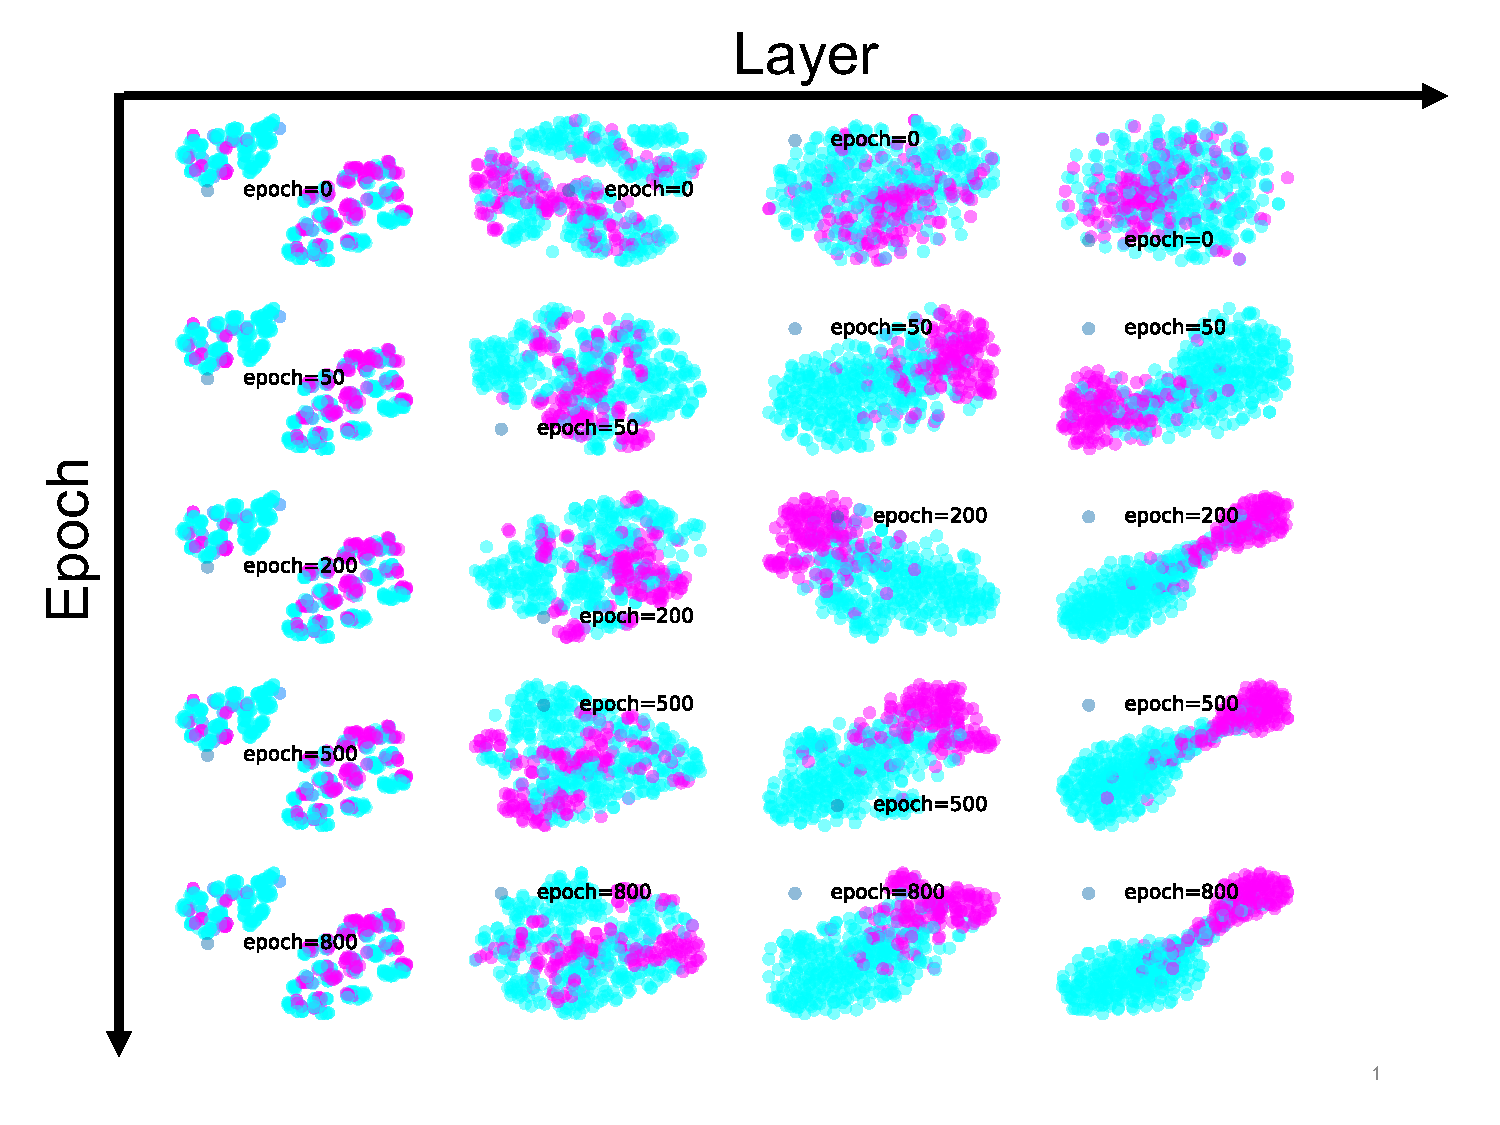
\includegraphics[width=8cm]{neural_networks/images/rep_learning}}; }] (Xp) at (3,3) {};}
\end{tikzpicture}

\end{frame}
\begin{frame}[t]{Conclusions}
In summary:
\vspace{1cm}
\pause{}
\begin{enumerate}
	\item Neural network models provide model complexity `on tap'\pause{}
	\item Backpropagation allows easy access to derivatives  \pause{}
	\item We can understand neural networks as automatic feature selection/transformation, followed by linear regression
\end{enumerate}

\end{frame}

\begin{frame}{ANN example}
jupyter notebook: \url{github.com/jpjanet/ML-chem-workshop/blob/master/notebooks/ANN.ipynb}
\end{frame}